\section{The whiteboard photographs}\label{app:photos}

Two photographs show the same lecture board at slightly different angles \cite{whiteboard1,whiteboard2}.
They are read together.
\Cref{fig:board} reproduces both.

\begin{figure}[ht]
\centering
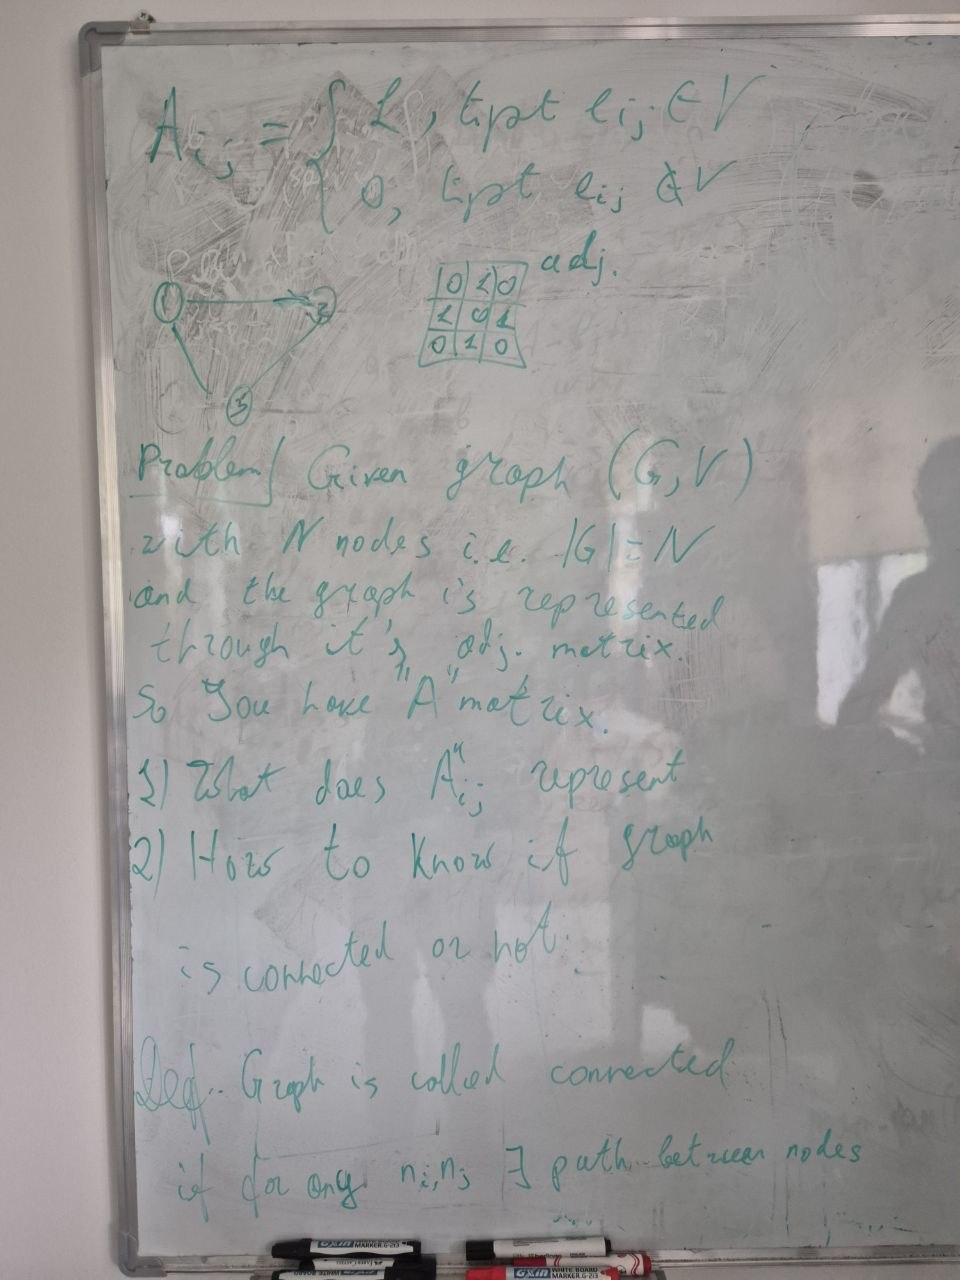
\includegraphics[width=0.46\textwidth]{sources/whiteboard-1.jpg}\hfill
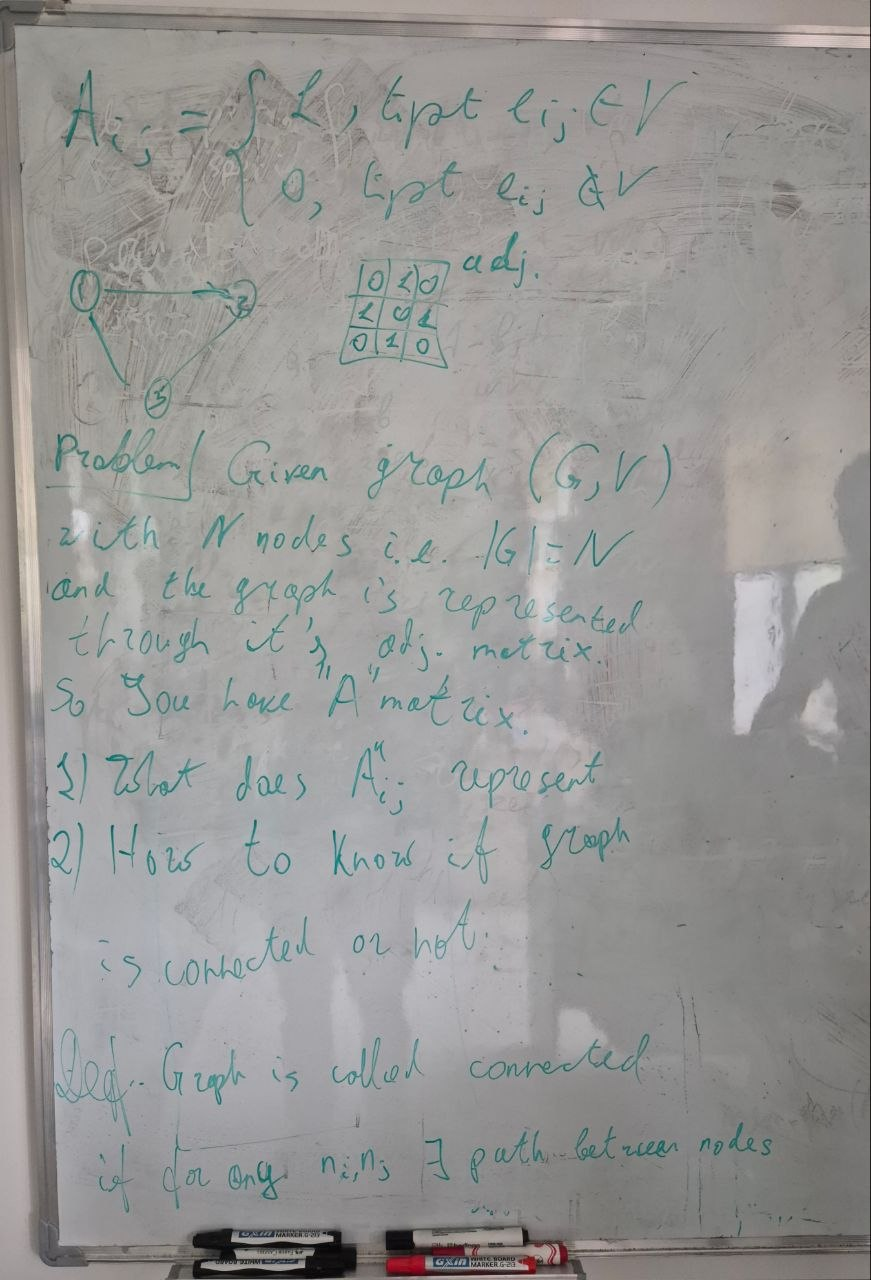
\includegraphics[width=0.46\textwidth]{sources/whiteboard-2.jpg}
\caption{The two photographs of the lecture board \cite{whiteboard1,whiteboard2}. A reflection of a person is visible on the right.}\label{fig:board}
\end{figure}

\paragraph{Transcription in reading order.}
\begin{enumerate}
\item $A_{ij}=1$ if $e_{ij}\in V$, and $0$ if $e_{ij}\notin V$; the board's $V$ is the edge set \cite{whiteboard1,whiteboard2}.
\item A drawing with vertices labelled $1,2,3$, and next to it a matrix labelled ``adj.'' with rows $0\,1\,0$ / $1\,0\,1$ / $0\,1\,0$.
\item ``Problem. Given graph $(G,V)$ with $N$ nodes i.e.\ $|G|=N$ and the graph is represented through it's adj.\ matrix. So you have $A$ matrix.''
\item ``1) What does $A_{ij}$ represent'', with a small mark above $A$.
\item ``2) How to know if graph is connected or not.''
\item ``Def. Graph is called connected if for any $n_i,n_j$ there exists a path between nodes.''
\end{enumerate}

\paragraph{Clearly visible.}
All the prose above, the matrix entries, and the vertex labels.

\paragraph{Likely interpretation.}
The mark above $A$ is an exponent $k$ (interpretation, qualified: the assignment text asks about $A^k$, but in both photographs the mark looks like a small $n$ or a pair of quotation marks).
The arrowhead on the line $1$--$2$ is a stray mark, because the matrix is symmetric and the problem is about undirected graphs (interpretation).

\paragraph{Unclear or in conflict.}
The drawing shows a line from $1$ to $2$ with an arrowhead at $2$, a line from $1$ to $3$, and a line from $2$ to $3$, which would be three edges, while the matrix encodes only the edges $1$--$2$ and $2$--$3$ \cite{whiteboard1,whiteboard2}.
Edge by edge: the edge $1$--$2$ is in both; the edge $2$--$3$ is in both; the edge $1$--$3$ is in the drawing only.
The paper follows the matrix and reports the mismatch.
